% Options for packages loaded elsewhere
\PassOptionsToPackage{unicode}{hyperref}
\PassOptionsToPackage{hyphens}{url}
\PassOptionsToPackage{dvipsnames,svgnames,x11names}{xcolor}
%
\documentclass[
  11pt,
  letterpaper,
  DIV=11,
  numbers=noendperiod]{scrartcl}

\usepackage{amsmath,amssymb}
\usepackage{iftex}
\ifPDFTeX
  \usepackage[T1]{fontenc}
  \usepackage[utf8]{inputenc}
  \usepackage{textcomp} % provide euro and other symbols
\else % if luatex or xetex
  \usepackage{unicode-math}
  \defaultfontfeatures{Scale=MatchLowercase}
  \defaultfontfeatures[\rmfamily]{Ligatures=TeX,Scale=1}
\fi
\usepackage[]{mathpazo}
\ifPDFTeX\else  
    % xetex/luatex font selection
\fi
% Use upquote if available, for straight quotes in verbatim environments
\IfFileExists{upquote.sty}{\usepackage{upquote}}{}
\IfFileExists{microtype.sty}{% use microtype if available
  \usepackage[]{microtype}
  \UseMicrotypeSet[protrusion]{basicmath} % disable protrusion for tt fonts
}{}
\makeatletter
\@ifundefined{KOMAClassName}{% if non-KOMA class
  \IfFileExists{parskip.sty}{%
    \usepackage{parskip}
  }{% else
    \setlength{\parindent}{0pt}
    \setlength{\parskip}{6pt plus 2pt minus 1pt}}
}{% if KOMA class
  \KOMAoptions{parskip=half}}
\makeatother
\usepackage{xcolor}
\usepackage[margin=1in]{geometry}
\setlength{\emergencystretch}{3em} % prevent overfull lines
\setcounter{secnumdepth}{-\maxdimen} % remove section numbering
% Make \paragraph and \subparagraph free-standing
\makeatletter
\ifx\paragraph\undefined\else
  \let\oldparagraph\paragraph
  \renewcommand{\paragraph}{
    \@ifstar
      \xxxParagraphStar
      \xxxParagraphNoStar
  }
  \newcommand{\xxxParagraphStar}[1]{\oldparagraph*{#1}\mbox{}}
  \newcommand{\xxxParagraphNoStar}[1]{\oldparagraph{#1}\mbox{}}
\fi
\ifx\subparagraph\undefined\else
  \let\oldsubparagraph\subparagraph
  \renewcommand{\subparagraph}{
    \@ifstar
      \xxxSubParagraphStar
      \xxxSubParagraphNoStar
  }
  \newcommand{\xxxSubParagraphStar}[1]{\oldsubparagraph*{#1}\mbox{}}
  \newcommand{\xxxSubParagraphNoStar}[1]{\oldsubparagraph{#1}\mbox{}}
\fi
\makeatother


\providecommand{\tightlist}{%
  \setlength{\itemsep}{0pt}\setlength{\parskip}{0pt}}\usepackage{longtable,booktabs,array}
\usepackage{calc} % for calculating minipage widths
% Correct order of tables after \paragraph or \subparagraph
\usepackage{etoolbox}
\makeatletter
\patchcmd\longtable{\par}{\if@noskipsec\mbox{}\fi\par}{}{}
\makeatother
% Allow footnotes in longtable head/foot
\IfFileExists{footnotehyper.sty}{\usepackage{footnotehyper}}{\usepackage{footnote}}
\makesavenoteenv{longtable}
\usepackage{graphicx}
\makeatletter
\def\maxwidth{\ifdim\Gin@nat@width>\linewidth\linewidth\else\Gin@nat@width\fi}
\def\maxheight{\ifdim\Gin@nat@height>\textheight\textheight\else\Gin@nat@height\fi}
\makeatother
% Scale images if necessary, so that they will not overflow the page
% margins by default, and it is still possible to overwrite the defaults
% using explicit options in \includegraphics[width, height, ...]{}
\setkeys{Gin}{width=\maxwidth,height=\maxheight,keepaspectratio}
% Set default figure placement to htbp
\makeatletter
\def\fps@figure{htbp}
\makeatother

\usepackage{booktabs}
\usepackage{longtable}
\usepackage{array}
\usepackage{multirow}
\usepackage{wrapfig}
\usepackage{float}
\usepackage{colortbl}
\usepackage{pdflscape}
\usepackage{tabu}
\usepackage{threeparttable}
\usepackage{threeparttablex}
\usepackage[normalem]{ulem}
\usepackage{makecell}
\usepackage{xcolor}
\makeatletter
\def\@maketitle{%
  \begin{center}%
  \let \footnote \thanks
    {\LARGE \@title \par}%
    {\large \@author \par}%
    {\large \@date}
  \end{center}%
  \par
  \vskip 1em}
\makeatother
\RedeclareSectionCommand[beforeskip=1ex plus -.2ex minus -.2ex,afterskip=.25ex plus -.1ex minus -.1ex]{section}
\RedeclareSectionCommand[beforeskip=1ex plus -.2ex minus -.2ex,afterskip=.25ex plus -.1ex minus -.1ex]{subsection}
\RedeclareSectionCommand[beforeskip=1ex plus -.2ex minus -.2ex,afterskip=.25ex plus -.1ex minus -.1ex]{subsubsection}
\raggedbottom
\usepackage{enumitem}
\setlist{nolistsep}
\KOMAoption{captions}{tableheading}
\makeatletter
\@ifpackageloaded{caption}{}{\usepackage{caption}}
\AtBeginDocument{%
\ifdefined\contentsname
  \renewcommand*\contentsname{Table of contents}
\else
  \newcommand\contentsname{Table of contents}
\fi
\ifdefined\listfigurename
  \renewcommand*\listfigurename{List of Figures}
\else
  \newcommand\listfigurename{List of Figures}
\fi
\ifdefined\listtablename
  \renewcommand*\listtablename{List of Tables}
\else
  \newcommand\listtablename{List of Tables}
\fi
\ifdefined\figurename
  \renewcommand*\figurename{Figure}
\else
  \newcommand\figurename{Figure}
\fi
\ifdefined\tablename
  \renewcommand*\tablename{Table}
\else
  \newcommand\tablename{Table}
\fi
}
\@ifpackageloaded{float}{}{\usepackage{float}}
\floatstyle{ruled}
\@ifundefined{c@chapter}{\newfloat{codelisting}{h}{lop}}{\newfloat{codelisting}{h}{lop}[chapter]}
\floatname{codelisting}{Listing}
\newcommand*\listoflistings{\listof{codelisting}{List of Listings}}
\makeatother
\makeatletter
\makeatother
\makeatletter
\@ifpackageloaded{caption}{}{\usepackage{caption}}
\@ifpackageloaded{subcaption}{}{\usepackage{subcaption}}
\makeatother

\ifLuaTeX
  \usepackage{selnolig}  % disable illegal ligatures
\fi
\usepackage{bookmark}

\IfFileExists{xurl.sty}{\usepackage{xurl}}{} % add URL line breaks if available
\urlstyle{same} % disable monospaced font for URLs
\hypersetup{
  pdftitle={DSC 365: Introduction to Data Science},
  colorlinks=true,
  linkcolor={blue},
  filecolor={Maroon},
  citecolor={Blue},
  urlcolor={Blue},
  pdfcreator={LaTeX via pandoc}}


\title{DSC 365: Introduction to Data Science}
\usepackage{etoolbox}
\makeatletter
\providecommand{\subtitle}[1]{% add subtitle to \maketitle
  \apptocmd{\@title}{\par {\large #1 \par}}{}{}
}
\makeatother
\subtitle{Course Policies and Syllabus, Fall 2024}
\author{}
\date{}

\begin{document}
\maketitle


\subsection{Course Policies and Syllabus, Spring
2025}\label{course-policies-and-syllabus-spring-2025}

\begin{longtable}[]{@{}
  >{\raggedright\arraybackslash}p{(\columnwidth - 2\tabcolsep) * \real{0.6861}}
  >{\raggedright\arraybackslash}p{(\columnwidth - 2\tabcolsep) * \real{0.3139}}@{}}
\toprule\noalign{}
\endhead
\bottomrule\noalign{}
\endlastfoot
Instructor: Alex Kunin & Office: Hixson-Lied 439 \\
Email:
\href{mailto:alexkunin@creighton.edu?subject=DSC\%365}{alexkunin@creighton.edu}
& \\
Lecture: Tuesday/Thursday 9:30-10:45 & Hixson-Lied 522 \\
\begin{minipage}[t]{\linewidth}\raggedright
Office Hours:\\
Mondays\\
Wednesdays\\
or by appointment (send an email!)\strut
\end{minipage} & \begin{minipage}[t]{\linewidth}\raggedright
\hfill\break
12:00-1:00 and 2:30-4\\
2:00-4:00\\
\strut
\end{minipage} \\
\end{longtable}

\subsubsection{Class Materials}\label{class-materials}

\textbf{Textbook}: \emph{Modern Data Science with R}

\begin{itemize}
\tightlist
\item
  Baumer (ISBN-13: 978-0367191498) -
  \url{https://mdsr-book.github.io/mdsr3e/}
\end{itemize}

\textbf{Software}

\begin{itemize}
\tightlist
\item
  R: \url{https://cran.r-project.org}
\item
  RStudio: \url{https://www.rstudio.com/}
\end{itemize}

\subsubsection{Course Description}\label{course-description}

\emph{Introduction to Data Science} uses computing tools to gather,
manage and analyze large and complex data sets. Topics include data
wrangling and formatting, web scraping, data analysis, statistical
modeling techniques, text mining and language processing.

DSC 365 also addresses Department of Mathematics Learning Objectives 2
and 4:

\begin{itemize}
\tightlist
\item
  Objective 2. Communication in Mathematics: The ability to communicate
  effectively in both oral and written forms while applying their
  mathematical skills. Students will learn the basic language of proof
  and counterexample. Students will organize and present significant
  ideas and calculations in written form.
\item
  Objective 4. Breadth and Depth: Students will develop an awareness of
  the breadth and depth of mathematics. This will include an awareness
  of historical and contemporary contexts in which mathematics is
  practiced. They will develop critical perspectives of the inherent
  limitations of the discipline.
\end{itemize}

\subsubsection{Objectives}\label{objectives}

There are six major topics in Introduction to Data Science:

\begin{itemize}
\tightlist
\item
  Exploratory data analysis, including data visualization using ggplot2.
\item
  Data wrangling and formatting using the tidyverse set of R libraries.
\item
  Data acquisition using web-scraping and APIs.
\item
  Statistical modeling techniques such as regression models and
  clustering techniques.
\item
  Text mining and language processing.
\item
  Reproducible research and dynamic programming using R/RStudio.
\end{itemize}

We'll work through many of these topics simultaneously. This class is
all about building skills and techniques to begin your data science
journey.

\subsubsection{Class Preparation}\label{class-preparation}

\textbf{General}: Students should come to each class meeting prepared to
write and talk intelligently about the material. This means watching any
required videos or reading any required materials before class. The
assignments will require thought and analysis, which cannot be had in 15
minutes or less. Give yourself adequate time to read carefully, to think
and reflect, to sleep on it, then maybe glance it over before class.

\textbf{Computing and Software}: Computing is an essential part of
modern statistical practice: meaningful data science is impossible
without computing. We will be using the open-source statistical
computing language R and user interface program RStudio to graph
probability distributions, calculate probabilities, demonstrate
theoretical results, and investigate complex problems. You should plan
to bring a charged laptop to class every day. Further, please make sure
you turn the sound off so that you do not disrupt other students'
learning. In addition, if you are doing anything other than taking notes
or looking at course materials I will revoke your ability to use it.

\textbf{Textbook}: The textbook provides background material that is
meant to supplement lectures. Lecture notes indicate what sections of
the text you should read if you choose to do so.

\textbf{Attendance}: All students are expected to come to class prepared
to learn and actively participate. However, if you must be absent check
BlueLine for assignments, announcements, and any other information you
may have missed. If you must be absent for one of the Mini-Project
Presentation days, please make all efforts to notify me ahead of time
and be prepared to present official documentation of the reason for your
absence (doctor's note, etc.).

If chronic mental or physical health issues may/will lead to repeated
absences or absences beyond course syllabus expectations, please contact
\href{https://www.creighton.edu/student-success/student-accessibility-services}{Student
Accessibility Services} located in the Old Gym (suite 437; 402-280-2166)
to ensure accommodations are granted and communicated with your
instructors.

\subsubsection{Course Assessment}\label{course-assessment}

Your grade in DCS365 will contain the following components.

\begin{enumerate}
\def\labelenumi{\arabic{enumi}.}
\item
  Weekly Labs (35\%): Each (typically) Thursday we'll start a lab
  designed to explore new techniques for working with data. These labs
  are designed to take about 2-3 hours to complete, so you'll most
  likely need to finish them outside of class. Labs are due in BlueLine.
  The lowest score will be dropped. You can talk about the assignment in
  a group, but each student will submit assignments individually unless
  otherwise noted.
\item
  Mini-Projects (45\%): We will divide one project into four mini steps
  to help you understand the process for data analysis. These projects
  will be completed on your own. One Mini-Project will be due every 2-3
  weeks (typically on Thursdays). The grading of the mini-projects will
  be a combination of presentation, peer review and instructor grading.
  Here are the details:
\end{enumerate}

\begin{itemize}
\tightlist
\item
  Presentation for mini project 1 (5\%)
\item
  Written submission for mini project 2, instructor grading (10\%)
\item
  Self-Reflection on Peer Review/Written submission for mini project 3,
  instructor grading (5\%)
\item
  Written submission for mini project 4, instructor grading (15\%)
\item
  Presentation for mini project 4, peer grading (5\%)
\item
  Presentation for mini project 4, instructor grading (5\%)
\end{itemize}

\begin{enumerate}
\def\labelenumi{\arabic{enumi}.}
\setcounter{enumi}{2}
\tightlist
\item
  Analysis plan (20\%): Your Final Project will represent a complete
  exploration of a large-scale data project, suitable for use in a
  portfolio of your work. Final Projects are due on day of university
  assigned final exam date (Tuesday December 10 at 11:59pm). You will
  have the option to either complete this project on your own or in a
  group of two.
\end{enumerate}

All assignments must be readable, and when appropriate, all work must be
shown to receive credit (meaning code included). A missed work will
result in a score of zero unless you contact me before class with a note
from your advisor, physician, organization, or coach stating explicit
reasons for your absence. Adjustments may be made in extraordinary
circumstances. Please make sure you upload the correct assignment. A 10
point penalty will occur for improperly uploaded assignments (ie. wrong
assignment, blank file).

\subsubsection{Course Grades}\label{course-grades}

Your overall course score will be a weighted average of each element as
noted above. Grades may be curved at the instructors' discretion. A
letter grade will be assigned based on:

\begin{longtable}[]{@{}
  >{\raggedright\arraybackslash}p{(\columnwidth - 10\tabcolsep) * \real{0.1667}}
  >{\raggedright\arraybackslash}p{(\columnwidth - 10\tabcolsep) * \real{0.1667}}
  >{\raggedright\arraybackslash}p{(\columnwidth - 10\tabcolsep) * \real{0.1667}}
  >{\raggedright\arraybackslash}p{(\columnwidth - 10\tabcolsep) * \real{0.1667}}
  >{\raggedright\arraybackslash}p{(\columnwidth - 10\tabcolsep) * \real{0.1667}}
  >{\raggedright\arraybackslash}p{(\columnwidth - 10\tabcolsep) * \real{0.1667}}@{}}
\toprule\noalign{}
\endhead
\bottomrule\noalign{}
\endlastfoot
\textbf{A}: 93 - 100 & \textbf{A-}: 90-92.9 & \textbf{B+}: 87-89.9 &
\textbf{B}: 83-86.9 & \textbf{B-}: 80-82.9 & \textbf{C+}: 77-79.9 \\
\textbf{C}: 73-76.9 & \textbf{C-}: 70-72.9 & \textbf{D}: 60-69.9 &
\textbf{F}: Below 60 & & \\
\end{longtable}

\subsection{Other Policies}\label{other-policies}

\textbf{Emails} : Sending email to your instructor should be treated as
professional communication. Students should not assume their emails will
be answered immediately, and should allow (at least) 24 hours for a
response.

\begin{itemize}
\item
  To increase the chances of a quick response, start the subject line
  with ``DSC365'' so that it is clear that the email pertains to this
  class.
\item
  If having an issue running code, please include the error and the line
  trying to run
\end{itemize}

\textbf{Office hours}: The purpose of office hours is to provide you
with an opportunity for additional conversation, guidance or help.
Please feel free to come to our office hours at the time designated
above. If you are not able to attend the office hour, \emph{please email
me to set up an appointment}.

\textbf{Grades and regrades}: Course grades will appear on BlueLine.
Each student is responsible for verifying his or her recorded scores on
an ongoing basis. If there is any homework question that you want to
request for a regrade, please come to the office hour or email me.
\emph{Any regrade request should be submitted within 1 week of the
homework being graded}

\textbf{Late Policy}: If you know you are to be absent for an
assignment, please work with me to complete it prior to your absence.
Work that is submitted late for any reason may be deducted 20\% per day
that it is late, and (in general) it will not be accepted after five (5)
days. However, please contact me if there is an emergent or unique
situation that keeps you from completing your work on time.

\subsubsection{Academic Honesty}\label{academic-honesty}

This course is governed by the Policy on Academic Honesty of the College
of Arts and Science. The CCAS policy on academic honesty can be found at
the link below.
\url{https://www.creighton.edu/fileadmin/user/CCAS/curriculum/CCAS\_Academic\_Honesty\_Policy\_.pdf}

You are encouraged to work together on homework labs and in-class
activities, but all work you submit must be your own (unless the
assignment specifically states otherwise).

Special Note: Academic Dishonesty also includes using unauthorized
sources for the completion of a particular assignment. For example, this
would include consulting old solutions, looking up solutions to problems
on the internet, using Google or Microsoft translate, or using other
resources like other textbooks or online services like Chegg.com or
other websites to complete your work. This also includes using any form
of generative AI to do entire assignments, though using it as a study
aide is allowed.

Any assignment turned in that fails to meet this policy on academic
honesty will be scored as a zero, and the College of Arts and Sciences
will be notified. Repeated violations of this policy will result in an
automatic failure of this course.

\subsection{Grade Appeal:}\label{grade-appeal}

If you feel that I have not followed the syllabus, you have a right to
appeal your final grade. As there are a number of requirements that must
be met in order to submit a formal grade appeal, I suggest you closely
read the
\href{https://catalog.creighton.edu/pharmacy-health-professions/administration-academic-policies/grade-appeals-policy/grade-appeals-policy.pdf}{policy}
(in the student handbook) before doing so.

\subsection{Class cancellation
statement:}\label{class-cancellation-statement}

If class is canceled I will notify you as soon as possible through
BlueLine. There are a variety of assignments in Blue Line that I will
use if class is canceled due to my own illness or emergent situation. If
I am not able to contact you for some reason, please watch for an email
from the chair of the department, Dr.~Pennington, or the department
administrative assistant Nicole Lakeman.

\subsubsection{Force Majeure Policy}\label{force-majeure-policy}

Creighton University may modify, suspend, or postpone any and all
activities and services immediately and without notice because of force
majeure causes beyond Creighton's control and occurring without its
fault or negligence including, but not limited to, acts of god, fire,
war, governmental action, terrorism, epidemic, pandemic, weather,
national emergencies, or other threats to the safety of students or
staff. Creighton may, at its option, alter the academic schedule or
provide alternate instruction modalities to meet course objectives and
competencies and program outcomes, including, but not limited to,
distance or remote learning, until such time as Creighton determines
normal operations may resume safely.

In the event of a disruption of normal classroom activities due to
emergencies such as a disease outbreak the format for this course may be
modified to enable completion of the course. In that event, you will be
provided an addendum to this syllabus that will supersede this version.

\subsubsection{ADA Statement}\label{ada-statement}

Creighton University is committed to providing a supportive educational
atmosphere for all students. Students requesting accommodations are
encouraged to contact the Office of Student Accessibility Services (SAS)
as soon as possible to discuss the request process and eligibility
requirements, as accommodations are not retroactive. If you believe that
you may qualify or have questions regarding accommodations, please visit
the
\href{https://www.creighton.edu/student-success/student-accessibility-services}{SAS
website} for more information.

\subsubsection{Take Care of Yourself}\label{take-care-of-yourself}

\textbf{Healthy Lifestyle:} Do your best to maintain a healthy lifestyle
by eating well, exercising, avoiding excessive drug and alcohol use,
getting enough sleep and taking some time to relax. This will help you
achieve your goals and cope with stress. Your mental health is more
important than your grade in this course. All of us benefit from support
during times of struggle. You are not alone. An important part of the
college experience is learning how to ask for help.

\textbf{Student Counseling Services:} If you or anyone you know
experiences any academic stress, difficult life events, or feelings like
anxiety or depression, I strongly encourage you to seek support. The
Office of Student Retention offers students assistance in navigating
their way at Creighton through support, resources and advising. Student
Counseling Services is also here to help: call 402-280-2735 and visit
their
\href{https://studentlife.creighton.edu/wellness/health-and-counseling/student-counseling-services}{website}.
Consider reaching out to us, a friend, faculty or family member you
trust for help getting connected to the support that can help. If the
situation is life threatening, call the police:

On campus: Creighton Public Safety: 402-280-2911; Off campus: 911

\subsubsection{Title IX, Harassment, and
Discrimination}\label{title-ix-harassment-and-discrimination}

Individuals who may have experienced harassment, discrimination, or an
incident of discrimination under Title IX (sexual assault, sexual
harassment, dating violence, stalking, sex discrimination, or pregnancy
discrimination) are encouraged to contact the Office of Title IX and
Civil Rights Compliance at 402-280-3189 or
\href{mailto:TitleIX@creighton.edu}{\nolinkurl{TitleIX@creighton.edu}}
(Omaha) or 602-812-4590 or
\href{mailto:TitleIXPHX@creighton.edu}{\nolinkurl{TitleIXPHX@creighton.edu}}
(Phoenix) to make a report or learn more about support services
available on campus.

Faculty members are required under Creighton policy to report Title IX
incidents to the Office of Title IX and Civil Rights Compliance to
ensure compliance with federal law, and to maintain the safety of the
campus community and its members. For more information, please visit the
Office of Title IX and Civil Rights Compliance.

Students with documented disabilities or those who are pregnant may
request accommodations from Student Accessibility Services. For more
information, contact 402.280.2166 or visit the Student Accessibility
Services page.

\subsubsection{Community Standards}\label{community-standards}

According to the Creighton University Student Handbook, all Creighton
students are to uphold the following standards of conduct:

\begin{enumerate}
\def\labelenumi{\arabic{enumi}.}
\tightlist
\item
  Act with professional, academic, and personal integrity.
\item
  Respect and promote the dignity of all persons.
\item
  Respect the policies and procedures of the Creighton University
  community and the rights of its members both on and off campus, as
  well as the just laws of the civic community and the rights of its
  members.
\item
  Support the personal, professional, academic, and vocational
  development of the members of the Creighton University Community.
\end{enumerate}

Upon the first violation of this standard of conduct, you will be
notified in writing (via university email) or via a face-to-face meeting
with the instructor. If the behavior continues, you will be asked to
leave class and referred to the Office of Community Standards and
Well-Being. You will not be permitted to return to class without
instructor permission.

For any conduct perceived to pose an immediate threat to the well-being
of others in the classroom, Public Safety (402-280-2911) shall be
contacted immediately for assistance, at the instructor's discretion.

\subsubsection{Confidential Services}\label{confidential-services}

Creighton University offers free, confidential support to students.

Violence Intervention and Prevention (VIP) Center 402.280.3794

Student Counseling Services 402.280.2735

\subsubsection{Important Univeristy
Dates:}\label{important-univeristy-dates}

\begin{itemize}
\tightlist
\item
  Monday January 20 -- Martin Luther King, Jr.~Day -- no classes
\item
  Tuesday January 21 -- last day to ADD classes
\item
  Thursday January 23 at 4:30 pm -- last day to DROP classes without a
  ``W''
\item
  Monday February 10 -- last to change to audit or P/NP
\item
  Spring Break: March 10-14 -- no classes
\item
  Thursday April 3 -- last day to withdraw with a ``W''
\item
  Easter Recess April 18-21 -- no classes after 5pm on April 17th
\item
  Final semester examinations: May 8-14
\end{itemize}

\newpage

\subsubsection{Class Schedule and Topic
Outline}\label{class-schedule-and-topic-outline}

This schedule is tentative and subject to change. The most up-to-date
schedule is on Blueline.

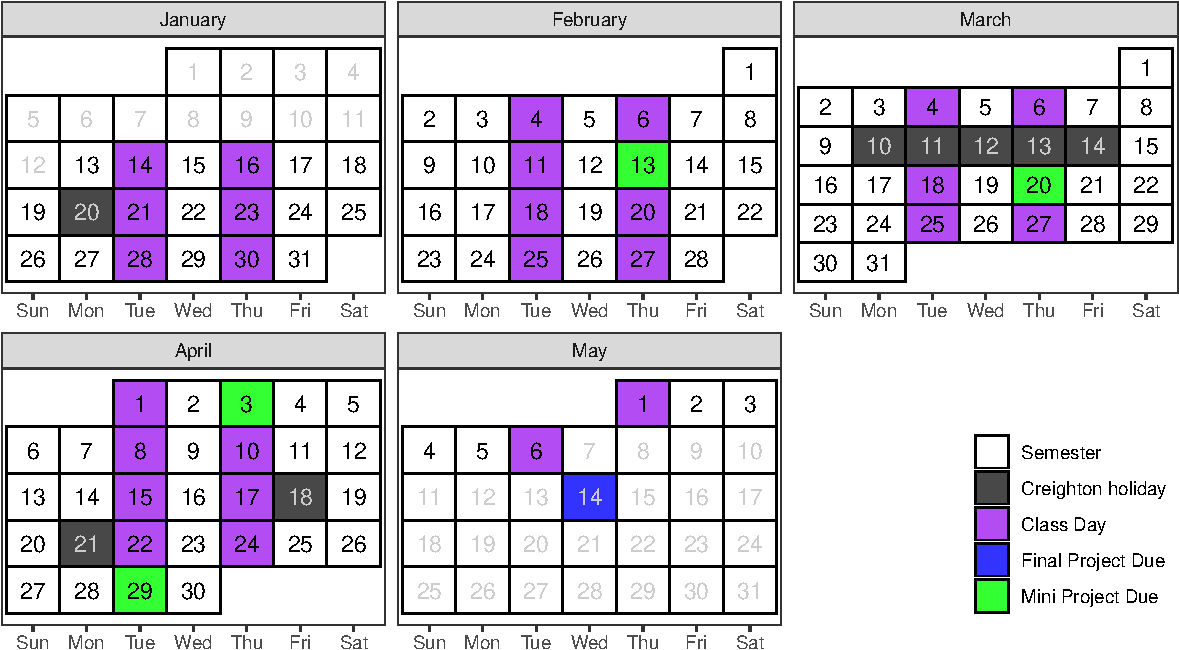
\includegraphics{figs/calendar.pdf}

\begin{longtable}[]{@{}llll@{}}
\caption{Tentative schedule of class topics and important due
dates}\tabularnewline
\toprule\noalign{}
Date & Tuesday & Thursday & Project \\
\midrule\noalign{}
\endfirsthead
\toprule\noalign{}
Date & Tuesday & Thursday & Project \\
\midrule\noalign{}
\endhead
\bottomrule\noalign{}
\endlastfoot
Jan 14, Jan 16 & Syllabus & Introduction to R & \\
Jan 21, Jan 23 & Basic R and Quarto & Lab 1 & \\
Jan 28, Jan 30 & Data Visualization & Lab 2 & MP 1 Relesase \\
Feb 4, Feb 6 & Data Wrangling & Lab 3 & \\
Feb 11, Feb 13 & Data Communication and Ethics & Present MP 1 & MP 1
Due \\
Feb 18, Feb 20 & Loops and Function Writing & Lab 4 & MP 2 Release \\
Feb 25, Feb 27 & Statistical Modeling & Statistical Modeling & \\
Mar 4, Mar 6 & Statistical Modeling & Lab 5 & \\
Mar 18, Mar 20 & Random Forests & Lab 6 & MP 2 due, MP 3 release \\
Mar 25, Mar 27 & KNN & Lab 7 & \\
Apr 1, Apr 3 & Text Data & Peer Review MP 3 & \\
Apr 8, Apr 10 & PCA & Clustering & MP3 Reflection due, MP4 release \\
Apr 15, Apr 17 & Lab 8 & Spatial Data & \\
Apr 22, Apr 24 & Web Scraping & Lab 9 & MP4 due, Final Project
Relsease \\
Apr 29, May 1 & Present MP 4 & Present MP 4 & \\
May 6 & Present MP 4 & & \\
May 14 & Present MP 4 & (8am, if needed) & Final Project Due \\
\end{longtable}




\end{document}
